\section{서론}
\label{sec:intro}

최근 연구에서는 Diffusion Large Language Models (dLLMs)~\cite{nie2025large,ye2025dream,zhu2025llada,zhao2025d1,labs2025mercury}가 급증하고 있다. dLLM은 sequence generation을 이산 denoising 과정으로 취급함으로써 지배적인 autoregressive (AR) 패러다임~\cite{brown2020language,achiam2023gpt}에 도전한다.
dLLM의 매력의 핵심은 이론적 유연성에 있으며, 이는 AR model의 엄격한 left-to-right causal chain에 비해 두 가지 뚜렷한 장점을 제공한다: 효율적인 parallel decoding과 arbitrary-order generation 능력이다.

parallel decoding의 효율성 이득은 이미 잘 확립되어 있지만~\cite{fastdllm,labs2025mercury,geminidiffusion,song2025seed,wu2025fast}, arbitrary-order generation의 함의는 상대적으로 덜 탐구되었다.
이론적으로 제약 없는 생성 순서는 고정된 autoregressive trajectory의 상위집합을 이루며, 더 발전된 문제 해결 능력을 열어 줄 잠재력을 가진다.
한편 일부 연구~\cite{ye2024beyond,kim2025train}는 스도쿠와 zebra puzzle 같은 특정 과제에서 non-sequential generation의 우수성을 입증했다.
이러한 성공과 이론적 가능성에 힘입어, 커뮤니티는 수학과 코딩 같은 \emph{일반 reasoning task}에서 유사한 고급 능력을 이끌어내기 위해 Reinforcement Learning (RL)을 점점 더 많이 채택해 왔다\footnote{
    우리는 이러한 도메인이 폭넓은 실용적 유용성과 reasoning model의 핵심 지능을 벤치마킹하는 중심적 역할을 지닌다는 점에서 \emph{일반 reasoning}의 주요 대표로 초점을 맞춘다.
    }~\cite{zhao2025d1,wang2025spg,gong2025diffucoder,rojas2025improving,ou2025principled}.

이 연구에서 우리는 반직관적인 관찰을 제시한다: 이러한 일반 reasoning task에서는 arbitrary-order generation이 RL로 이끌어낼 수 있는 reasoning 잠재력을 확장하기보다 오히려 좁힐 수 있다.
이를 엄밀히 평가하기 위해 우리는 solution space의 coverage를 측정하는 Pass@$k$~\cite{chen2021evaluating}를 사용한다.
최근 연구들은 RL이 주로 base model의 분포를 날카롭게 만드는 역할을 한다고 시사한다. 따라서 base model의 Pass@$k$ 성능은 RL 학습 후 모델이 달성 가능한 reasoning 한계에 대한 효과적인 proxy가 된다~\cite{yue2025does,liu2025prorl}.
이 지표 아래에서 우리는 LLaDA-Instruct~\cite{nie2025large}를 사용하여 arbitrary-order generation의 reasoning 잠재력을 표준 AR decoding과 비교한다.
Figure~\ref{fig:teaser}(왼쪽)에 보이듯, dLLM을 표준 AR order로 제한하면 유연한 counterpart보다 \emph{더 높은} Pass@$k$, 그리고 결과적으로 더 높은 reasoning boundary를 산출하는 경향이 있다.

\begin{figure}[t]\centering
    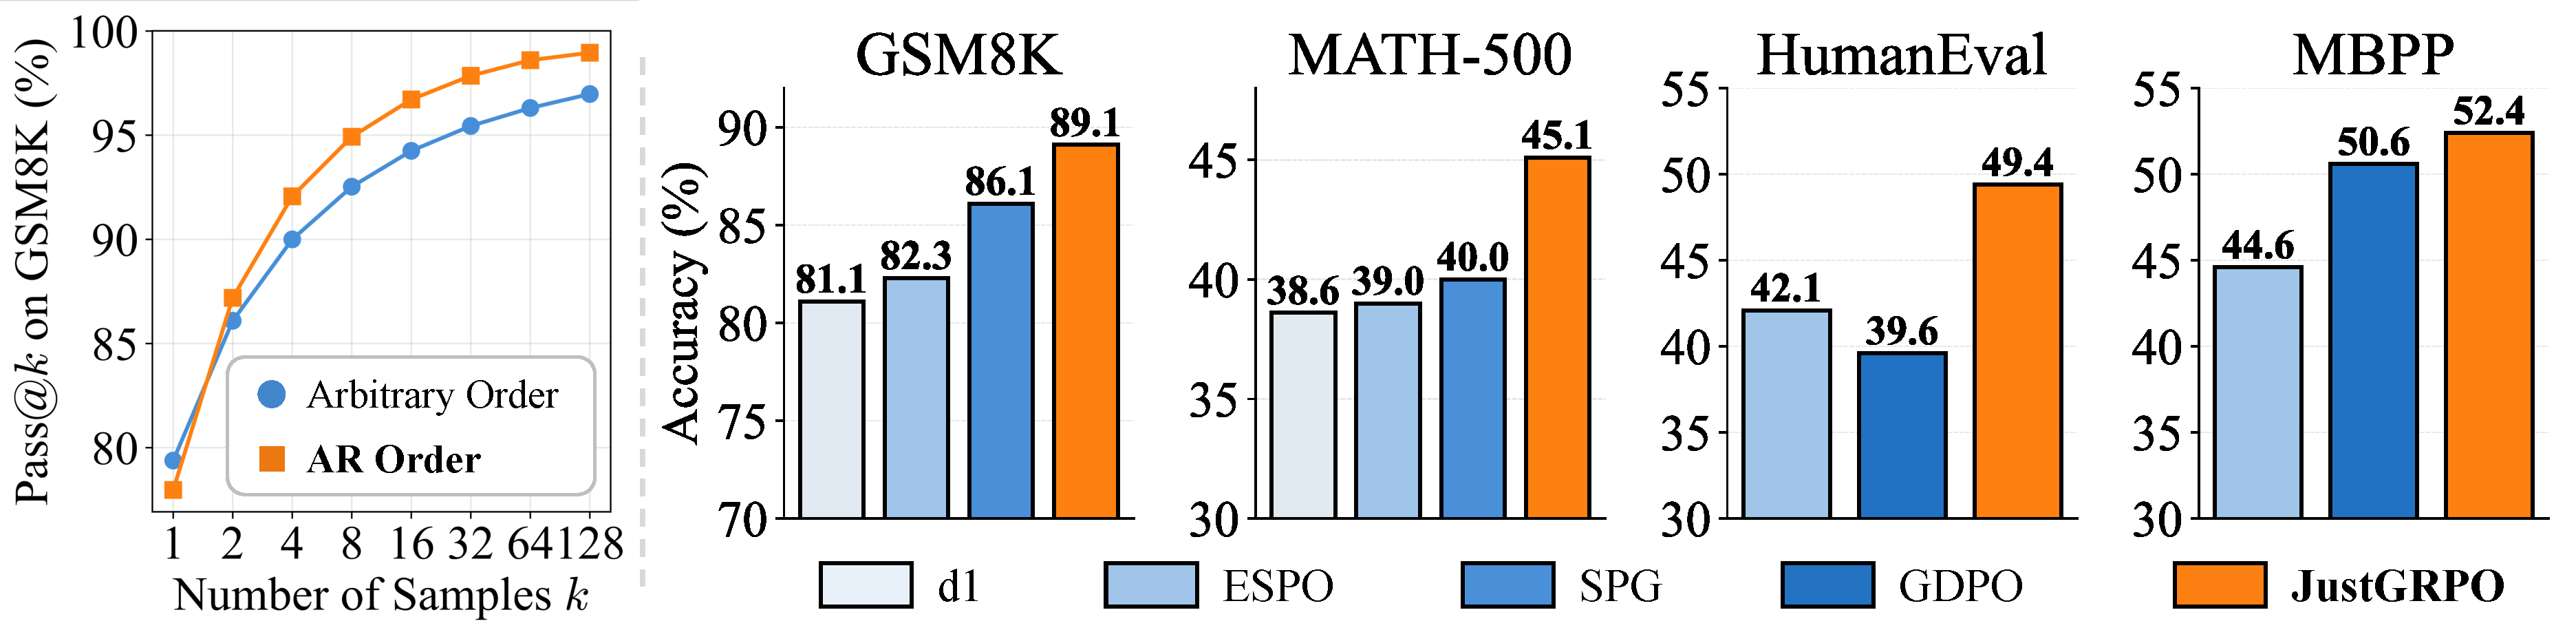
\includegraphics[width=\linewidth]{figures/teaser.pdf}
    \caption{
    \textbf{더 적은 유연성이 더 나은 reasoning 잠재력을 연다.}
    \emph{왼쪽}: dLLM을 표준 Autoregressive (AR) order로 제한하면 reasoning solution space가 확장되는 반직관적인 현상을 관찰한다.
    \emph{오른쪽}: 이에 동기를 받아 우리는 ``\textbf{JustGRPO}''를 제안한다. arbitrary-order adaptation을 포기하고 단지 GRPO를 채택함으로써, dLLM의 reasoning capability를 더 효과적으로 이끌어낸다. 결과는 생성 길이 256에서 LLaDA-Instruct~\cite{nie2025large}에 대해 보고했다. Baseline 결과는 해당 논문에서 인용했다. 또한 Table~\ref{tab:controlled_comparison}에는 맞춘 설정에서 재현한 결과도 포함한다.
    \label{fig:teaser}
    }
\end{figure}



이 반직관적인 관찰은 서로 다른 순서가 uncertainty를 처리하는 방식과 밀접하게 관련된다.
\begin{wrapfigure}{r}{0.52\textwidth}
    \centering
    \vskip -0.12in
    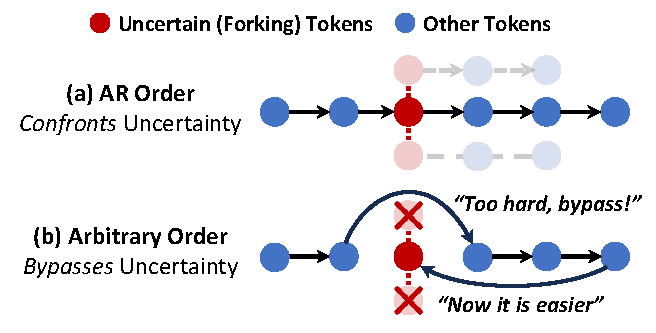
\includegraphics[width=\linewidth]{figures/illustrate.pdf}
    \vskip -0.10in
    \caption{
        \textbf{uncertainty에 맞서기 \emph{vs.} 우회하기.}
        (a) \textbf{AR order}는 uncertain token에서 결정을 강제함으로써 reasoning space를 보존한다.
        (b) \textbf{Arbitrary order}는 uncertainty를 우회하고 더 쉬운 token을 먼저 해결한다.
        미래 context가 확립되면, 원래의 branching 가능성은 사실상 pruning된다.
        \label{fig:illustrate}
    }
    \vskip -0.12in
\end{wrapfigure}
reasoning은 본질적으로 균일하지 않다. reasoning은 드문드문 나타나는 ``forking token''에 달려 있으며, 이는 보통 ``Therefore''나 ``Since'' 같은 연결어로서 단순히 문장을 이어 가는 것이 아니라 논리적 trajectory를 서로 다른 branch로 이끈다~\cite{wang2025beyond,cheng2025reasoning,huang2025low}.
이러한 fork에서 reasoning path는 갈라지며, 자연스럽게 entropy의 국소적 spike로 나타난다~\cite{wang2025beyond}.
표준 AR decoding은 모델이 이 uncertainty에 \emph{맞서도록} 강제한다(Figure~\ref{fig:illustrate}a).
바로 이러한 fork에서 sampling함으로써 모델은 서로 다른 reasoning path를 탐색할 수 있고, 따라서 생성된 rationale의 다양성을 보존한다.
반면 arbitrary-order generation은 모델이 이러한 어려운 결정을 \emph{우회할} 수 있게 한다(Figure~\ref{fig:illustrate}b).
이 유연성은 일반적으로 low-uncertainty token을 우선하기 위해 활용되며~\cite{nie2025large}, 이는 그 token으로 이어지는 연결어를 결정하기 전에 더 쉬운 부분에서 reasoning path를 사실상 고정한다.
모델이 우회한 fork를 infill하기 위해 돌아올 때쯤에는, 이미 확립된 미래 context가 그 ambiguity를 조기에 해소해 버린다.
우리는 이 현상을 \emph{entropy degradation}이라 부른다: fork에 원래 내재했던 high entropy가 억제되는 것이다.
결과적으로 모델은 더 이상 branching point를 탐색하는 것이 아니라, 사전에 결정된 gap을 잇도록 연결어를 맞추고 있을 뿐이다.





위 관찰은 이러한 일반 reasoning task에서 dLLM을 위한 RL을 재고하도록 동기를 부여한다.
현재 방법들은 arbitrary-order 유연성을 보존하는 것이 필수적이라는 가정 아래 작동한다. 이러한 고수에는 큰 비용이 따른다. 알고리즘은 denoising trajectory의 combinatorial explosion~\cite{zhao2025d1,yang2025mmada,gong2025diffucoder}과 다루기 어려운 marginal likelihood~\cite{ou2025principled,wang2025spg}에 맞서야 하며, 부정확한 approximation~\cite{wang2025spg,ou2025principled,rojas2025improving}에 의존할 수밖에 없다.
하지만 arbitrary order가 target task의 잠재력을 이끌어내는 데 필수적이지 않거나 심지어 해롭다면, 이러한 복잡성은 불필요할 수 있다.

이를 위해 우리는 \textbf{JustGRPO}를 통해 단순성으로 돌아갈 것을 제안한다.
우리는 일반 reasoning task의 reasoning 잠재력을 이끌어내는 데 복잡한 diffusion-specific RL adaptation이 반드시 필요한 것은 아님을 보인다.
대신 RL 학습 중 dLLM을 단순히 AR policy로 취급함으로써 효과적으로 달성할 수 있다. 이를 통해 표준 GRPO~\cite{shao2024deepseekmath}를 수정 없이 적용하여, 그렇지 않았다면 다루기 어려운 optimization을 잘 정의된 과제로 바꾼다.
중요하게도, 이 AR formulation은 더 나은 exploration을 위해 RL 학습 중에만 ``scaffold'' 역할을 한다.
dLLM의 고유 architecture는 그대로 유지된다. \eg, causal masking을 부과하지 않으므로 bidirectional attention과 discrete diffusion formulation이 보존된다.
그 결과 \textit{reasoning ability의 elicitation}(sequential exploration의 이점을 얻음)과 \textit{inference execution}(dLLM의 parallel decoding 이점을 얻음)이 분리된다. 


단순함에도 불구하고 JustGRPO는 놀라울 정도로 효과적이다.
이는 강한 결과(\eg, GSM8K에서 89.1\% 정확도, MATH-500에서 45.1\%)를 달성하며, 복잡한 diffusion-specific RL adaptation에 의존하는 방법들과 비교해도 우수하다(Table~\ref{tab:main_results}).
더 중요하게는 Figure~\ref{fig:eb_sampler_comparison}에 보이듯, AR-trained model은 parallel decoding과 완전히 호환된 상태로 남아 있어, AR exploration을 통해 획득한 reasoning capability가 dLLM의 대표적인 inference efficiency를 희생할 필요가 없음을 시사한다.

